\documentclass[12pt]{article} % Document type.
\usepackage[a4paper, margin=2cm]{geometry} % Paper format.
\usepackage{textcomp}
\usepackage{amsmath}
\usepackage{graphicx} % Insert images.
\usepackage{caption}% Provides many ways to customise the captions in floating environments like figure and table, and cooperates with many other packages
\usepackage{subcaption}% Subfigures
\usepackage[utf8]{inputenc} % Accept different input encodings.
\usepackage[brazilian]{babel} % Language pack and special characters, respectively.
\usepackage{indentfirst} % Indents first paragraph in each section.
\usepackage{amsmath}% Provides various features to facilitate writing math formulas and to improve the typographical quality of LaTex output.
\usepackage{pdfpages} % Add images as annex pages in the PDF.
\usepackage{amssymb} %Add mathematical symbols
\usepackage{siunitx}
\usepackage{svg}
\usepackage{url}% Make URL links
\renewcommand{\thesection}{\arabic{section}}% Set \section as the major separation unit.
\newcommand{\comment}[1]{}
\usepackage[nottoc]{tocbibind}% References
\usepackage[rightcaption]{sidecap}
\usepackage{wrapfig}
\usepackage{array}
\usepackage{wrapfig}
\usepackage{multirow}
\usepackage{tabu}
\usepackage{steinmetz} %Phasors
\usepackage{pdfpages} % Add images as annex pages in the PDF.

% Table configuration
\setlength{\tabcolsep}{0.2cm}
\renewcommand{\arraystretch}{1.3}

\setlength{\jot}{10pt}% Definindo uma distância padrão entre as equações ao usar \\

\usepackage{hyperref} % make a clickable Summary
\hypersetup{
    colorlinks=false, %set true if you want colored links
    linktoc=all,     %set to all if you want both sections and subsections linked
}

\usepackage[section]{placeins} % To use \FloatBarrier and prevent images to jump out of it's section or subsection

%====================================
% ---------CAPA----------------------
%====================================

\title{
        \uppercase{Analyse du problème \\Balance à N Plateaux \\ avec l'algorithme backtracking} \\
    {\large Algorithme et Complexité} \\
    {\large Université de Lorraine - ENSEM ISN 2A}
}

\date{\vfill 01 janvier 2023}


\author{
  Déric Augusto França de Sales \\
  \texttt{32219632} \\
  \texttt{deric.sales@ufv.br}
  }

\begin{document}
\maketitle
\thispagestyle{empty}
\pagebreak

% \tableofcontents
% \thispagestyle{empty}
% \pagebreak

\setcounter{page}{1}
%=======================================
%-----------------1---------------------
%=======================================
\FloatBarrier
\section{le problème Balance à deux Plateaux}
%======================================

%- apresentar o algoritmo (não o programa, o pseudocódigo, talvez um diagrama)
%- explicar como o algoritmo funciona

Traditionnellement le problème est constituée d'une balance d'assiettes, qui doit être équilibrée à partir d'une quantité M de poids à N plateaux. Pour illustrer, nous allons d'abord considérer un système où la balance comporte deux plateaux qui doivent être équilibrés. Les plateaux sont équidistants du centre de la balance et physiquement les poids exercent un couple sur le bras de la balance qui supporte le plateau (figure \ref{fig:scale}). Le système ne sera en équilibre lorsque le poids du côté gauche sont en équilibré avec le poids du côté droit. Si les poids ne sont pas équilibrés, les couples générés par les deux côtés ne s'annuleront pas et le côté le plus lourd descendra. Ainsi, le problème vise à positionner les M corps qui présentent des poids différents sur le côté droit ou gauche de la balance, en recherchant l'équilibre maximal. 

\FloatBarrier
\begin{figure}[!h]
\centering
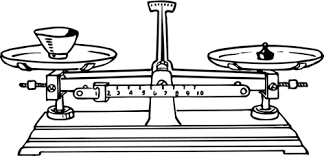
\includegraphics[width = 0.5\linewidth]{imgs/scale2.png}
\caption{Représentation d'une balance de plateaux.}
\label{fig:scale}
\end{figure}
\FloatBarrier

Il ne sera pas toujours possible d'obtenir un équilibre parfait (cas où les poids du côté droit et du côté gauche sont égaux), mais il cherche à réduire la différence entre les poids qui se trouvent des deux côtés de la balance. Ainsi, en modélisant le problème mathématiquement, on aura :

\begin{align}
    &w_i = \left[w_1, w_2, ..., w_m \right] \label{eq:wi} \\
    &x_i = \begin{cases}
    0 \;\;\; \text{si $w_i$ est placé sur le côté gauche de l'échelle};\\
    1 \;\;\; \text{si $w_i$ est placé sur le côté droit de l'échelle}.
    \end{cases} \label{eq:xi}
\end{align}

Où $w_i$ (\ref{eq:wi}) c'est le vecteur de $m$ poids, et $x_i$ (\ref{eq:xi}) le vecteur représentant la direction (droite ou gauche) dans laquelle le poids est positionné sur la balance. Une solution idéale est trouvée lorsque les poids sont parfaitement équilibrés entre les côtés droit et gauche de la balance, illustrée par la relation \ref{eq:equilibre}.

\begin{equation}
    \sum_{i=1}^m w_i x_i = \sum_{i=1}^m w_i (1- x_i)
    \label{eq:equilibre}
\end{equation}

Étant donné un ensemble arbitraire de n poids, il n'y a aucune garantie qu'une solution au problème existe. Une solution existe toujours si, au lieu d'équilibrer les balances, le but est de minimiser la différence entre les poids totaux des plateaux de gauche et de droite. Ainsi, à travers le vecteur \ref{eq:wi}, l'objectif sera la minimisation de $\delta$, comme le montre la relation \ref{eq:delta}, en considérant la contrainte que tous les poids de \ref{eq:wi} doivent être positionnés sur la balance.

\begin{equation}
    \delta = \left| \sum_{i=1}^m w_i x_i - \sum_{i=1}^m w_i (1 - x_i) \right|
    \label{eq:delta}
\end{equation}

%=======================================
%---------------------------------------
%=======================================
\section{résoudre le problème en codant un algorithme}
%======================================

Alors, allons y à tout suite analyser le problème en codant un algorithme. L'algorithme en question est chargé d'équilibrer les poids du vecteur W sur les plateaux droite et gauche. 
La fonction ``balance2Plateaux" (joint au dossier, ainsi que les autres fonctions créées) prend en entrée le tableau python $W$ qui contient une liste de nombres représentant les poids à équilibrer. 

\FloatBarrier
\begin{figure}[!h]
\centering
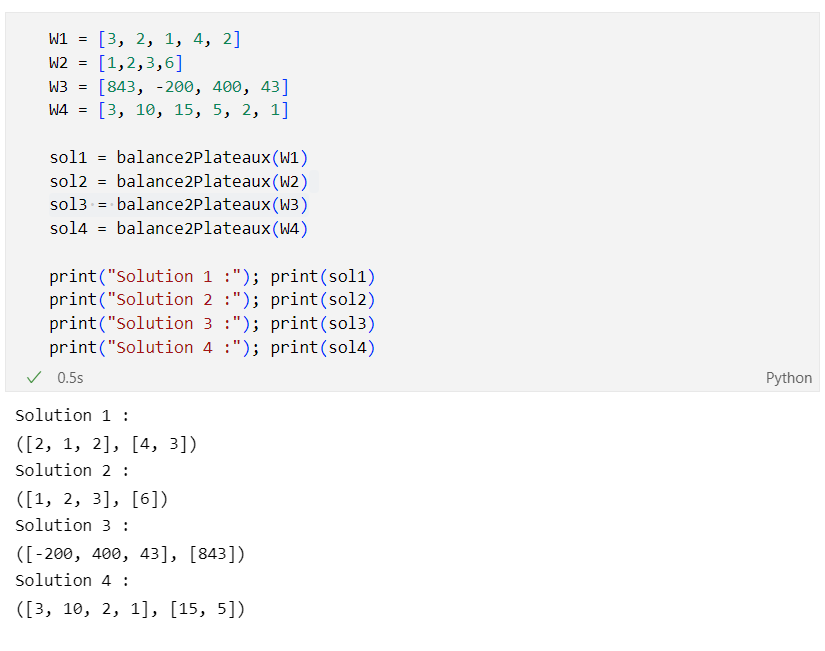
\includegraphics[width = 0.7\linewidth]{tests/1.png}
\caption{Test 1 effectué.}
\label{fig:test1}
\end{figure}
\FloatBarrier

Il est donc possible de constater que la fonction n'est pas efficace car elle ne fonctionne pas bien dans toutes les situations. Dans la solution 1 présentée par la Figure \ref{fig:test1}, la fonction donne comme réponse l'équilibrage des poids 2,1 et 2 dans un des plateaux de la balance et 4 et 3 dans l'autre plateau, étant donné que dans la solution optimale, l'équilibrage correct serait 4 et 2 dans un des plateaux et 3,1 et 2 dans l'autre, ayant 6 de poids total dans chaque plateau. La solution 2 est optimale, tandis que la solution 4 est également incorrecte. La solution 3 montre que la fonction ne traite pas bien non plus l'utilisation des numéros négatifs. 

Ainsi, nous pouvons voir que la première approche adoptée n'est pas très efficace, puisque la plupart du temps elle ne renvoie pas une solution correcte au problème, qui maximise l'équilibre entre les plaques. De plus, la fonction ne fonctionne qu'avec l'équilibrage entre deux plats, mais elle ne peut pas être généralisée à N plats. Pour résoudre ce problème, il est possible d'utiliser la technique du \textit{backtracking} (retour en arrière), qui crée un arbre de possibilités et parcourt les branches de l'arbre en essayant chaque possibilité.  Nous pouvons donc étendre le problème à N plats et appliquer la technique du \textit{backtracking} à sa solution.

%=======================================
%---------------------------------------
%=======================================
\section{résolution du problème Balance de M poids à N Plateaux à travers d'un algorithme de retour en arrière}
%======================================

Pour résoudre le problème dans le cas de N assiettes sur la balance, nous pouvons créer la variable $X$, qui sera une matrice chargée de stocker la solution au problème. Dans la matrice $X$, chaque ligne représente un plateau de balance différent, et chaque colonne représente un des éléments de poids du vecteur $W$. La matrice est aussi binaire, comme le vecteur $x$ dans la relation \ref{eq:xi}. C'est-à-dire que, si dans une case donnée s'il y a un numéro 1, cela signifie que le poids est sur cette échelle, et 0 sinon. Le schéma de la Figure \ref{fig:diagram} illustre la fonction créée pour résoudre ce problème. 

\FloatBarrier
\begin{figure}[!h]
\centering
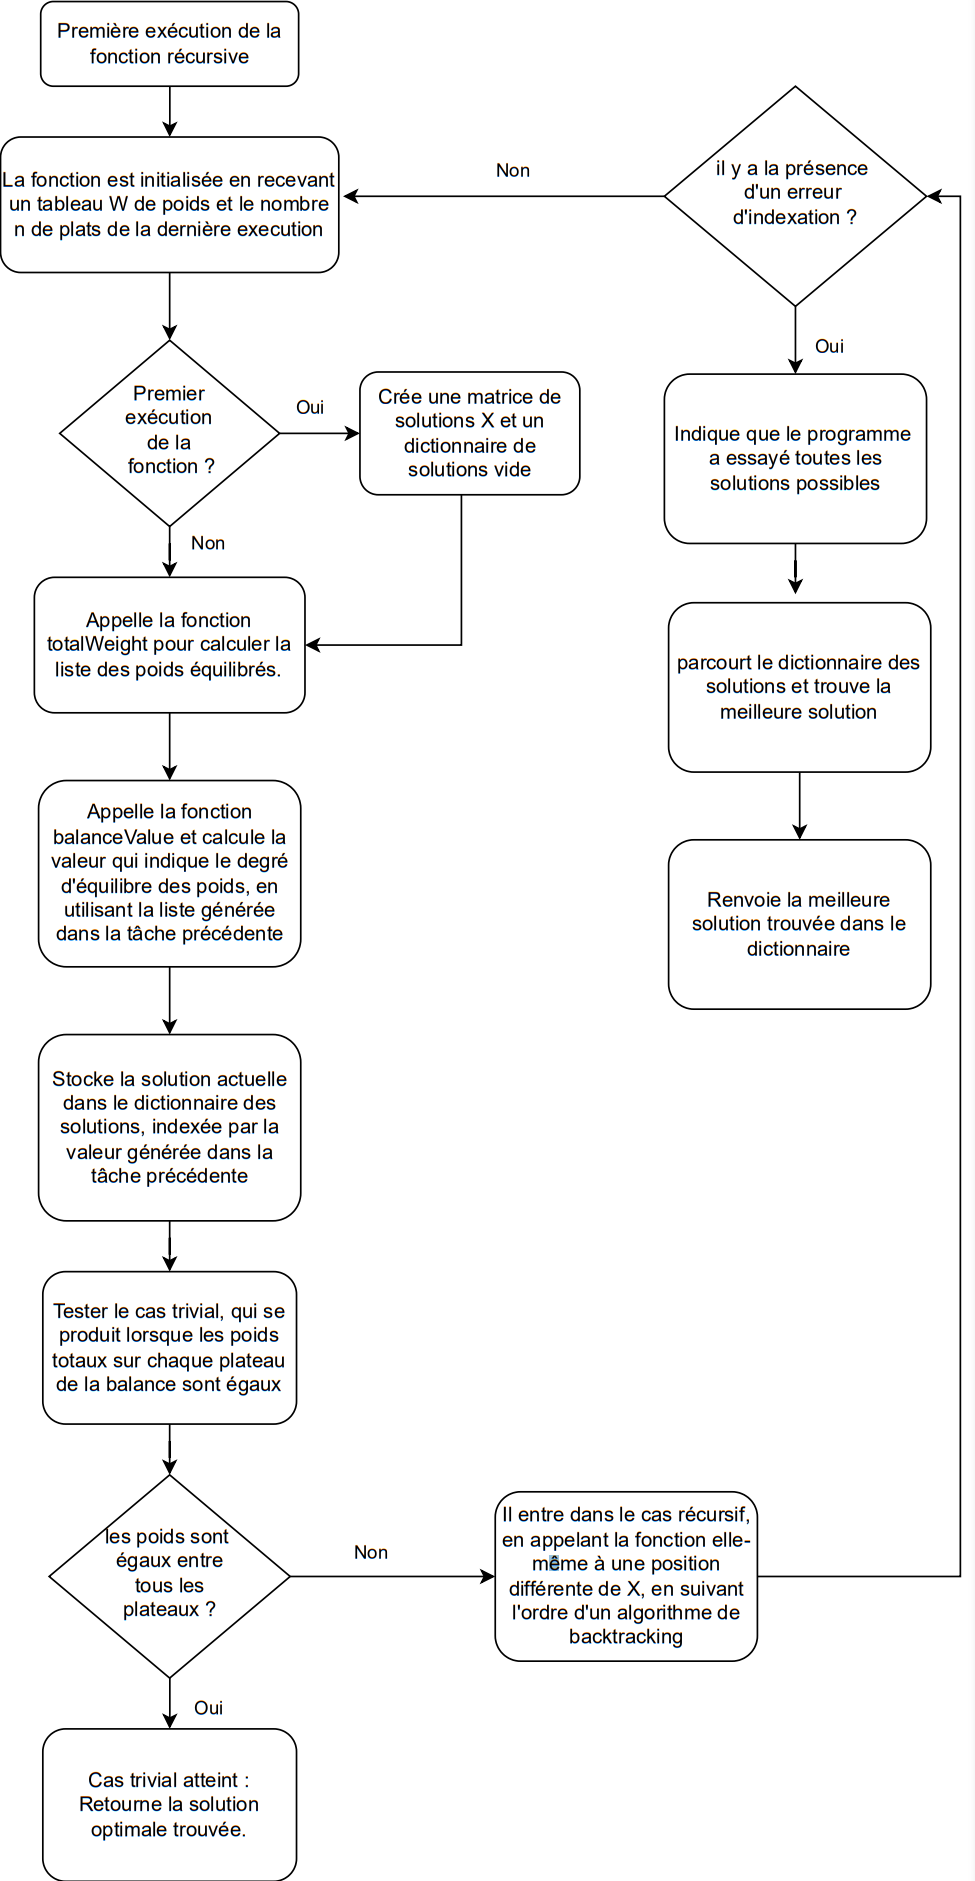
\includegraphics[width = 0.67\linewidth]{diagram/diagrama.png}
\caption{Diagramme de la fonction \textit{backtracking}.}
\label{fig:diagram}
\end{figure}
\FloatBarrier

La fonction de retour en arrière effectue ses tâches en utilisant d'autres fonctions. Nous allons d'abord expliquer plus en profondeur ces autres fonctions (elles sont jointes et commentées à la fin du fichier).

\vfill

 La fonction \textit{moveWeight} est chargée de déplacer les poids des plaques lorsqu'elle est appelée. C'est-à-dire qu'en passant la matrice de solution X et une colonne spécifique de cette matrice, qui indique l'un des éléments à déplacer, la fonction déplace l'élément vers la plateau suivante, ce qui est fait en déplaçant le numéro 1 vers la ligne inférieure de la colonne analysée. Ainsi, ce mouvement suit l'ordre d'un algorithme de \textit{backtracking}, en parcourant l'ensemble de l'arbre des solutions une par une. 

 \vfill

 Pour expliquer le fonctionnement de l'algorithme de \textit{backtracking}, nous allons prendre comme exemple un problème de 3 plateaux et 3 poids. Ce problème n'aurait pas de sens, car si nous avons trois plateaux et trois éléments, la seule solution possible serait de mettre un poids sur chaque plateau. Cependant, nous utiliserons cet exemple pour comprendre comment l'ordre d'exécution de l'algorithme est réalisé. La Figure \ref{fig:backtracking1} montre un arbre de solutions pour cet exemple, où les chiffres 0, 1 et 2 représentent le déplacement du chiffre 1 dans la matrice X dans chaque colonne. De plus, chaque niveau de l'arbre représente l'un des poids qui seront équilibrés. 

\vfill

\FloatBarrier
\begin{figure}[!h]
\centering
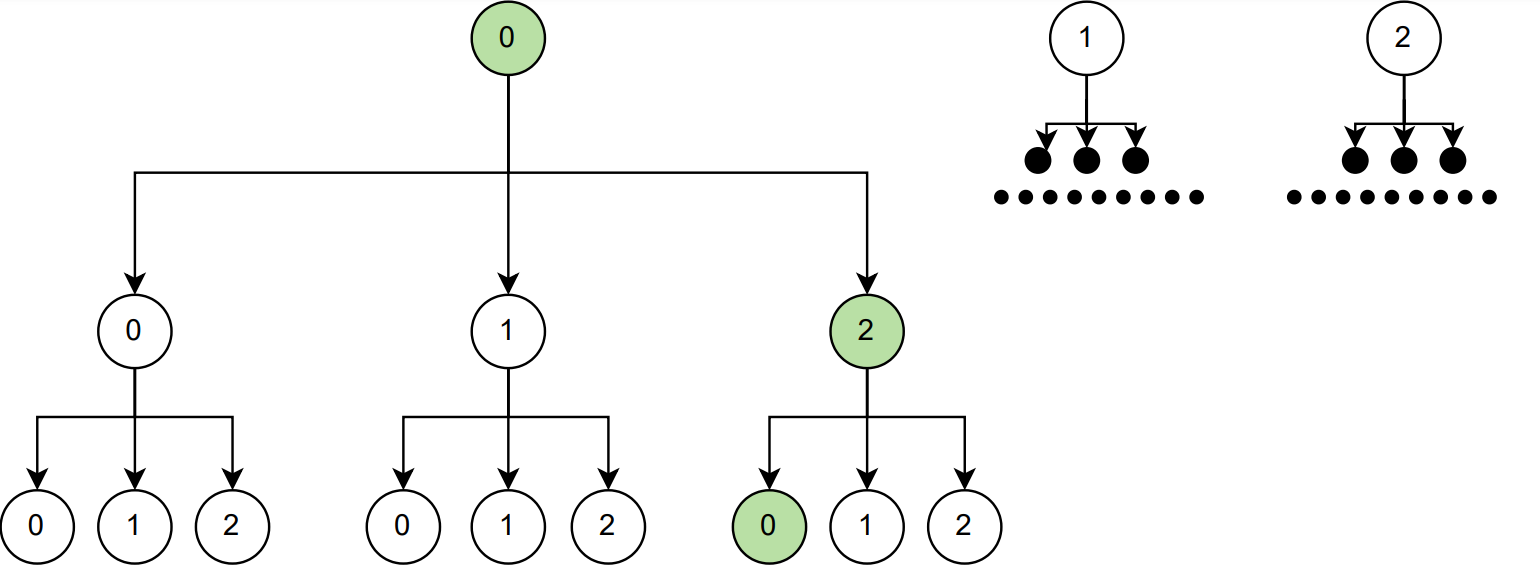
\includegraphics[width = 0.66\linewidth]{diagram/backtracking1.png}
\caption{Arbre des solutions simplifié pour n=3 et 3 poids, exemple 1.}
\label{fig:backtracking1}
\end{figure}
\FloatBarrier

\vfill

Ainsi, l'arbre de la Figure \ref{fig:backtracking1} générera la matrice X de la relation (\ref{X1}), où le premier élément du premier niveau de l'arbre a le mouvement 0, ce qui fait que le nombre 1 de la première colonne de la matrice reste dans la première ligne. De même, le deuxième poids aura un mouvement de 2, ce qui fait que le numéro 1 de la matrice X reste dans la troisième ligne, et le troisième poids, à son tour, a également un mouvement de 0, ce qui fait que le numéro 1 de la matrice X dans la dernière colonne reste dans la première ligne. Ainsi, dans cette solution, les poids 1 et 3 seront sur le premier plateau de la balance et le poids 2 sera sur le troisième plateau.

\vfill

\begin{equation}
           X = \begin{bmatrix}
            1 & 0 & 1 \\
            0 & 0 & 0 \\
            0 & 1 & 0
            \end{bmatrix} 
            \label{X1}
\end{equation}

\vfill

Afin de comprendre l'ordre d'exécution de l'algorithme de \textit{backtracking}, nous allons analyser la Figure \ref{fig:backtracking2}, qui montre l'itération suivante par rapport à la position dans l'arbre des solutions décrit par la Figure \ref{fig:backtracking1}. 

\vfill

\FloatBarrier
\begin{figure}[!h]
\centering
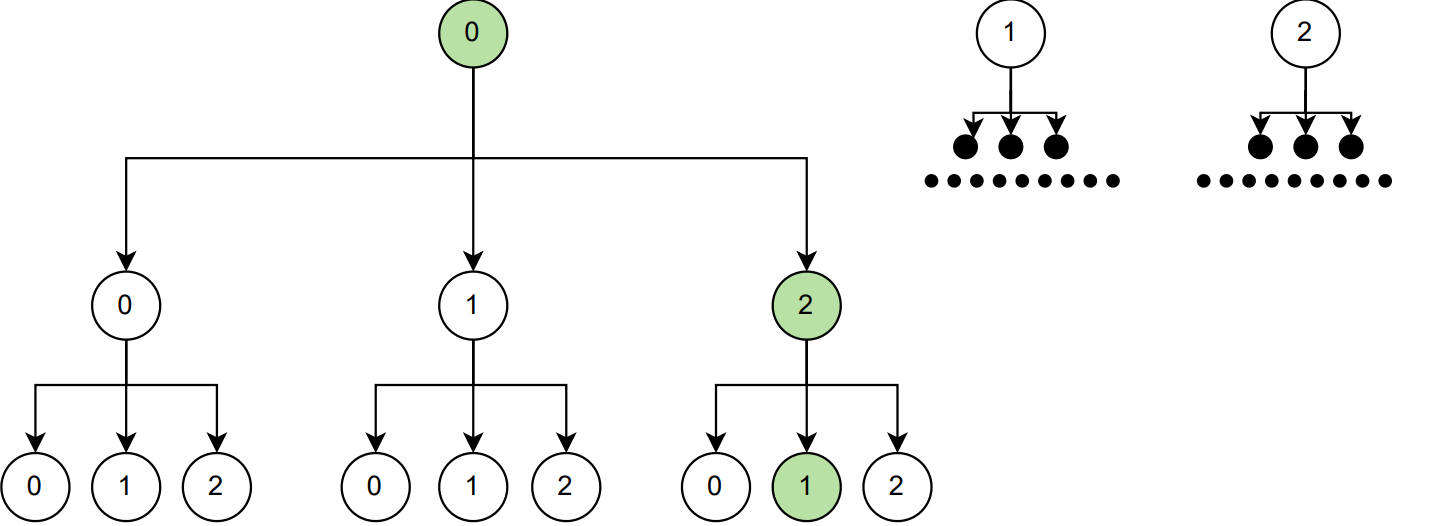
\includegraphics[width = 0.66\linewidth]{diagram/backtracking2.png}
\caption{Arbre des solutions simplifié pour n=3 et 3 poids, exemple 2.}
\label{fig:backtracking2}
\end{figure}
\FloatBarrier

\vfill

En passant à la branche suivante de l'arbre, nous allons générer la matrice des positions X de la relation (\ref{X2}). Ainsi, l'algorithme continue à fonctionner itération par itération, jusqu'à ce qu'il trouve une solution triviale, où les poids sont complètement équilibrés sur toutes les plateaux, ou jusqu'à ce qu'il essaie toutes les solutions et renvoie la meilleure. Ce qui a été expliqué pour n=3 (trois plateaux) et trois poids, vaut pour n plateaux et M poids, appartenant aux numéros naturels. 

\begin{equation}
           X = \begin{bmatrix}
            1 & 0 & 0 \\
            0 & 0 & 1 \\
            0 & 1 & 0
            \end{bmatrix} 
            \label{X2}
\end{equation}

Après avoir compris le fonctionnement de la fonction \textit{moveWeight} qui exécute l'ordre selon un algorithme de \textit{backtracking}, nous allons aborder les autres fonctions utilisées. La fonction \textit{totalWeigh} calcule le poids total dans chaque plateau et renvoie une liste avec tous ces poids totaux. La fonction \textit{weightDifference}, quant à elle, calcule la différence de poids entre tous ces poids totaux et renvoie une liste contenant toutes ces différences. Enfin, la fonction \textit{balanceValue} calcule la moyenne de ces différences, pour générer une valeur qui sera utilisée pour indiquer la qualité de la solution. Cette valeur sera utilisée comme critère de décision entre les solutions trouvées. 

Pour tester la fonction finale crée, on peut commencer par tester les mêmes exemples abordées par la Figure \ref{fig:test1}, avec deux plateaux. On peut conclure que la fonction \textit{backtrecking} donne la bonne réponse pour tout les cas, même avec des numéros négatifs. Si on teste d'autres cas, avec n=3 par exemple, on peut obtenir les résultats suivants :  

\vfill

\begin{align*}
    & W1 = [3, 2, 1, 4, 2] &W2 = [1, 2, 3, 6]\;\;\;\;\;\;\;\;\;\; & W3 = [3, 13, 9, 8, 1, 5]\\
    &X1 = \begin{bmatrix}
    1 & 0 & 1 & 0 & 0 \\
    0 & 1 & 0 & 0 & 1 \\
    0 & 0 & 0 & 1 & 0
    \end{bmatrix} 
    &X2 = \begin{bmatrix}
    0 & 0 & 0 & 1 \\
    0 & 0 & 1 & 0 \\
    1 & 1 & 0 & 0
    \end{bmatrix} \;\;\;\;\;\;\;\;\;\;
    &X3 = \begin{bmatrix}
    1 & 0 & 1 & 0 & 1 & 0 \\
    0 & 1 & 0 & 0 & 0 & 0 \\
    0 & 0 & 0 & 1 & 0 & 1
    \end{bmatrix} 
\end{align*}

\vfill

Nous pouvons noter que la fonction maximise l'équilibre dans tous les exemples, qu'il s'agisse d'une solution triviale ou non. Dans l'exemple de W1, la fonction atteint le résultat trivial ayant un poids total de 4 dans chaque plateau. L'exemple 3, quant à lui, présente un poids total de 13 dans chaque plateau.  

%=======================================
%---------------------------------------
%=======================================
\newpage
\section{analyse de la complexité de l'algorithme créé}
%======================================

Afin d'analyser la complexité de l'algorithme créé, nous allons d'abord analyser la complexité des fonctions utilisées dans la fonction de \textit{backtracking}. Tout d'abord, en analysant la complexité de la fonction \textit{totalWeight}, nous pouvons remarquer qu'elle présente deux boucles. L'une qui est exécutée en se référant au nombre de lignes de la matrice X, qui est égal au nombre de plateaux travaillés dans le problème, c'est-à-dire n. L'autre boucle s'exécute sur le nombre de colonnes de X, qui représente le nombre d'éléments à analyser, c'est-à-dire le nombre de poids du vecteur W. Nous appellerons le nombre de poids M. Ainsi, la fonction a un temps d'exécution O(n*M).

\vfill

La fonction \textit{weightDifference}, à son tour, présentera deux dimensions de boucles se référant à M, elle aura donc une complexité $O(M^2)$. La fonction \textit{balanceValue} présentera également cette même complexité, pour l'exécution de la fonction \textit{weightDifference} à l'intérieur.

\vfill

La fonction \textit{moveWeight}, quant à elle, présentera une complexité $(M-1)^n$ dans son exécution la plus défavorable, puisqu'elle suivra l'ordre de l'algorithme de \textit{backtracking}. On peut s'en rendre compte en analysant les arbres des figures \ref{fig:backtracking1} ou \ref{fig:backtracking2}, où chaque nœud multiplie le nombre de nœuds précédents. Dans l'exemple présenté dans les figures, nous aurons n = 3 et M = 3. Par conséquent, dans le pire des cas, si l'algorithme parcourt tout l'arbre, il sera exécuté $3^3 = 27$ fois.

\vfill

\FloatBarrier
\begin{figure}[!h]
\centering
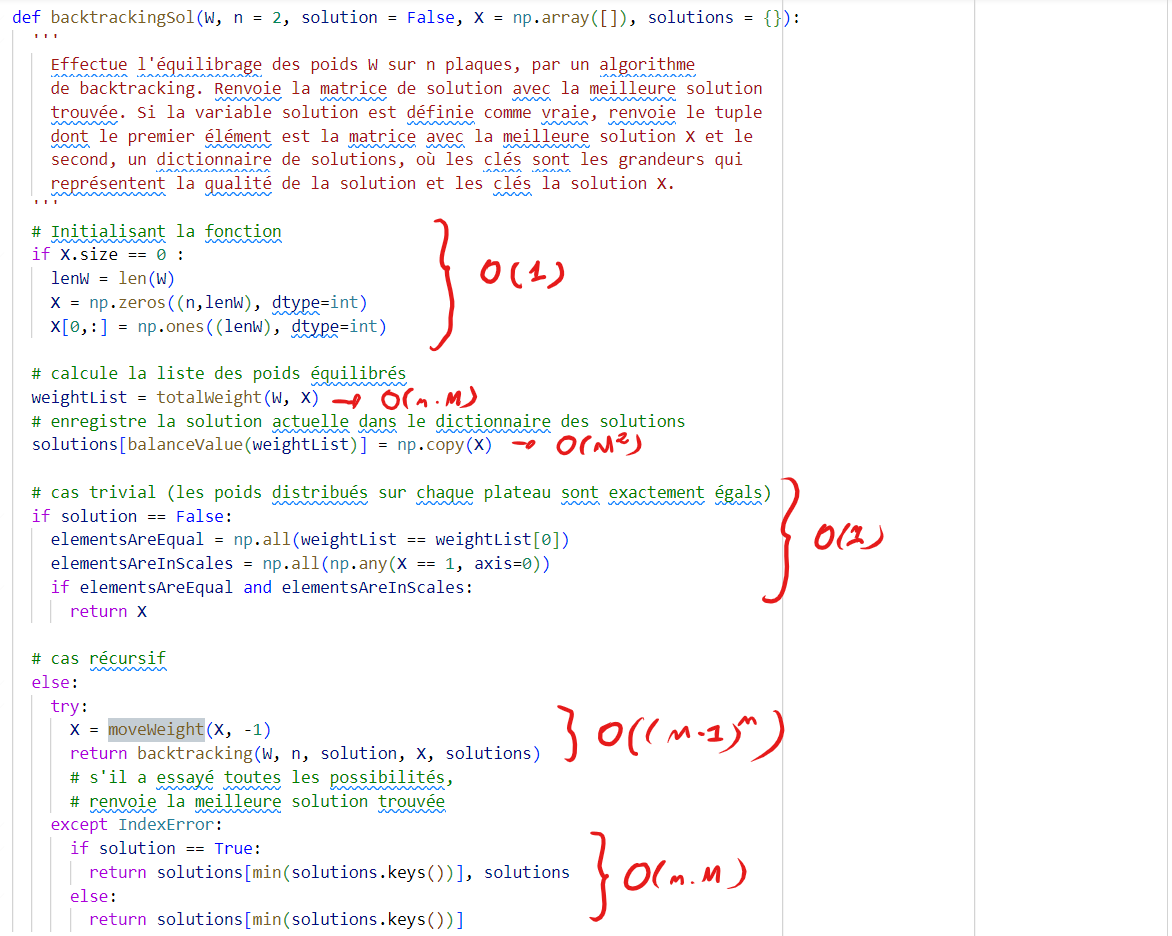
\includegraphics[width = 0.8\linewidth]{tests/comp.png}
\caption{Analyse de la complexité de la fonction de \textit{backtracking}.}
\label{fig:comp}
\end{figure}
\FloatBarrier

\vfill

En analysant la complexité de l'algorithme de \textit{backtracking} à travers la figure \ref{fig:comp}, nous pouvons voir que le terme avec le plus haut degré est $(M-1)^n$, donc ce sera la complexité de l'algorithme. On peut le simplifier pour obtenir $O(2^n)$, comme on l'écrit le plus souvent. On peut donc noter que pour les très grands termes, le nombre de plateaux de la balance compte plus pour le temps d'exécution de l'algorithme que le nombre de poids à équilibrer. 

%=======================================
%---------------------------------------
%=======================================
%\section{résolution du problème à travers d'un algorithme de type force brute}
%======================================



%=======================================
%---------------------------------------
%=======================================
%\section{résolution du problème à travers d'un algorithme de type backstepping}
%======================================





%=======================================
%---------------------------------------
%=======================================
%\section{résolution du problème à travers d'un algorithme de type force brute}
%======================================

%=======================================
%---------------------------------------
%=======================================
%\section{application à un problème réel}
%======================================

%- mostrar o algoritmo aplicado a alguma situação
%- mostrar o algoritmo implementado em alguma linguagem de programação

%=======================================
%---------------------------------------
%=======================================
%\section{limitations et comparaison avec la méthode de la force brute}
%======================================

%=======================================
%---------------------------------------
%=======================================
%\section{amélioration de la méthode}
%======================================

\FloatBarrier
\newpage

%==========================================
%-----REFERÊNCIAS-BIBLIOGRÁFICAS-----------
%==========================================
%\bibliographystyle{unsrt}
%\bibliography{referencias}
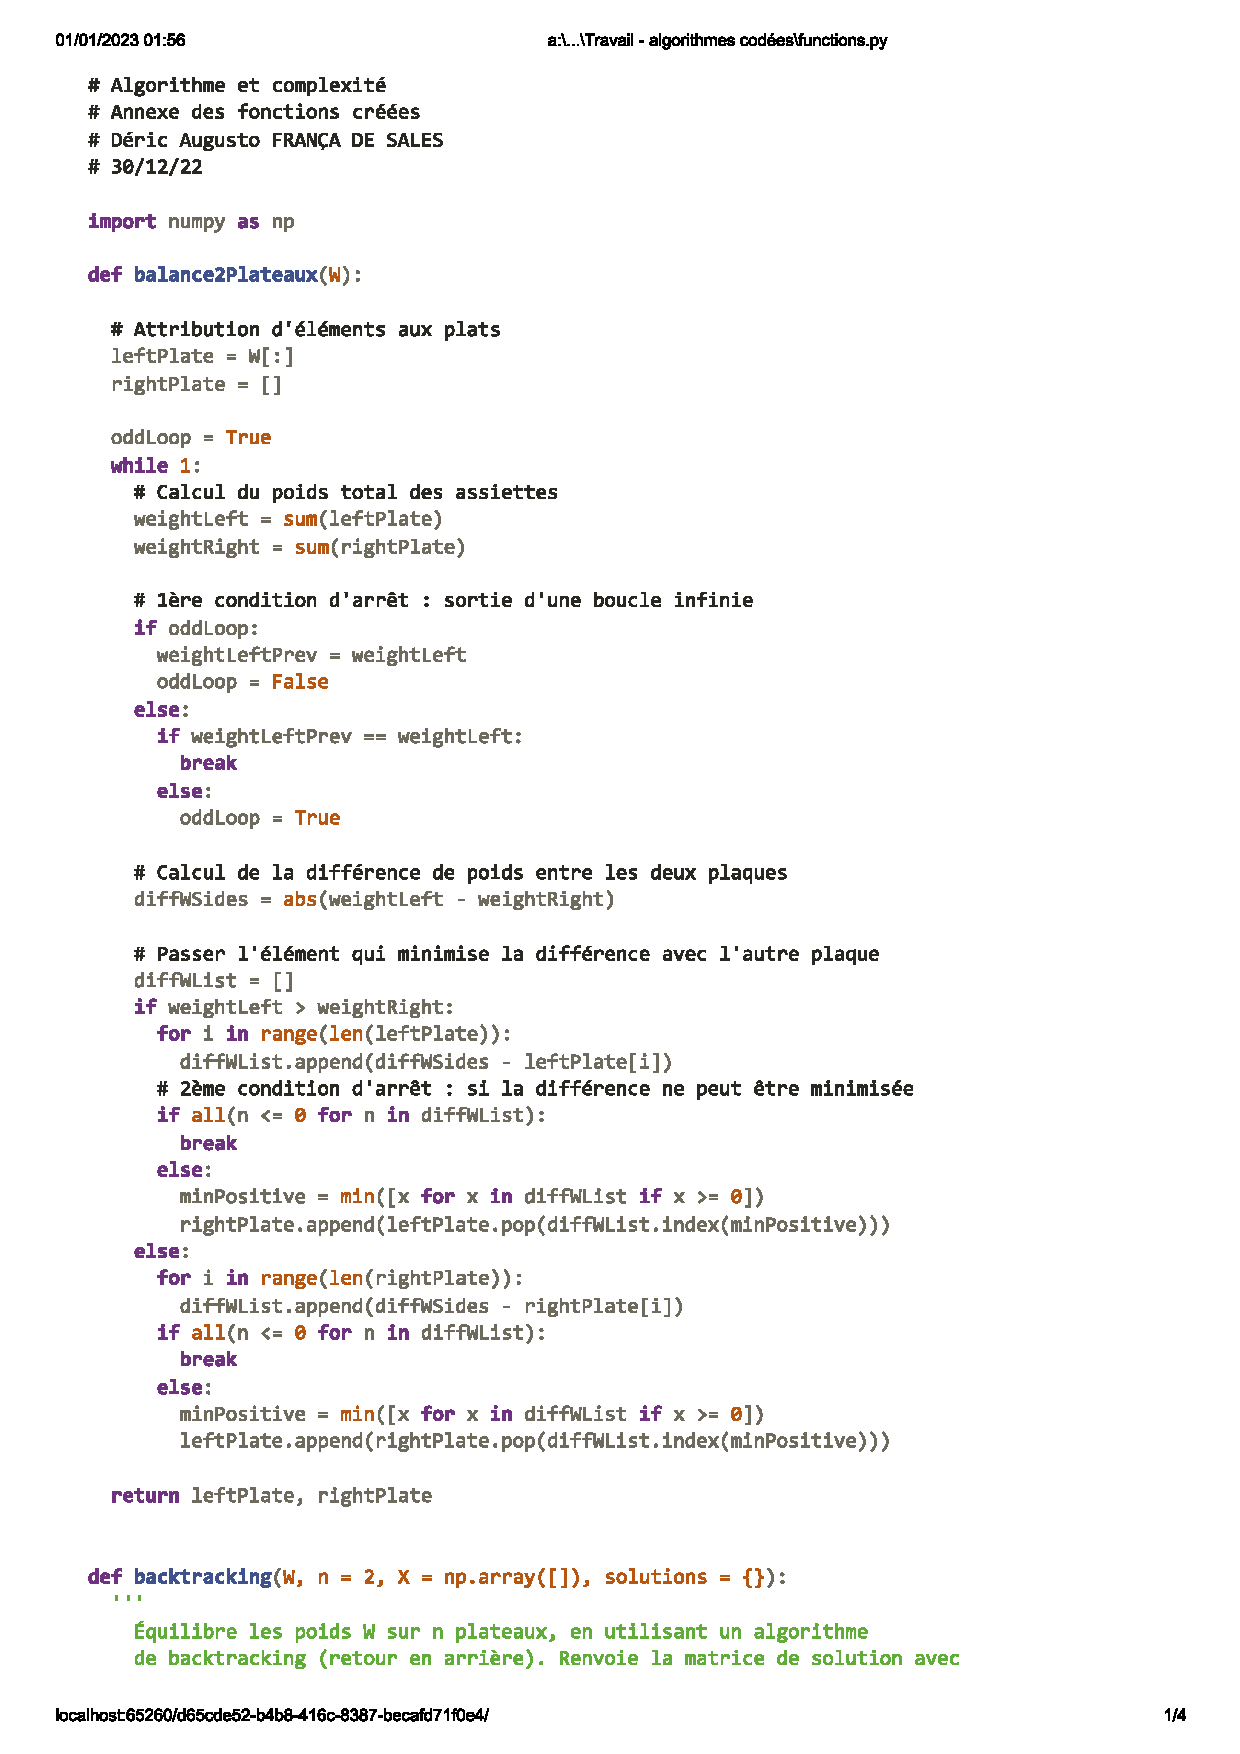
\includepdf[page ={1-}]{PDFscipts/anexo.pdf}
%==========================================

\end{document}

